\documentclass[10pt,a4paper]{beamer}
\usepackage[utf8]{inputenc}
\usepackage{amsmath}
\usepackage{amsfonts}
\usepackage{amssymb}
\usepackage[labelformat=empty]{subcaption}
\usepackage{graphicx}
\usepackage[dutch]{babel}
\usepackage{lmodern}
\usepackage{epstopdf}
\usepackage{ulem}
\usepackage{graphicx}
\usepackage[labelformat=empty]{caption}

\author{Falco Peijnenburg}
\usetheme{Warsaw}
%\setbeamertemplate{footline}{\insertframenumber/\inserttotalframenumber}


\title[Git crash course\hspace{40mm} \insertframenumber/\inserttotalframenumber]{Git crash course}


\begin{document}

% Title frame
\frame{\titlepage}

\setcounter{tocdepth}{1}
% Table of contents
\begin{frame}
\frametitle{Table of contents}
\tableofcontents[]
\end{frame}


\section{About git}
\subsection{What is git}
\begin{frame}{What is git}
\begin{itemize}
\item VCS (Version control systems)
\item SCM (Source code management)
\item Originally made by Linus Torvalds
\item Basically it makes your life easier when programming
\end{itemize}
\end{frame}

\subsection{Advantages git}

\subsection{By itself}
\begin{frame}{By itself}
\begin{itemize}
\item Distributed
\item Fast (both in speed of commands and workflow)
\item You can work offline
\item Forces you to have proper, structured workflow (and \textit{yes} this is good for everyone)
\item Has many features that are actually useful
\item It's useful even for people who work alone
\item Amazing branching implementation

\end{itemize}
\end{frame}
% multiple remotes, no problem

\subsection{Compared to Dropbox/Google Drive}
\begin{frame}{Compared to Dropbox/Google Drive}
\begin{itemize}
\item No more copying folders for an experimental feature/recode (seriously, this is ridiculous)
\item Work simultaneously without the \textit{utter} chaos of conflict files
\item You can very easily revert if you make a mistake
\item Better tracking of changes
\item The ability to find out when and by whom a bug was introduced
\end{itemize}
\end{frame}

\subsection{Compared to SVN}
\begin{frame}{Compared to SVN}
\begin{itemize}
\item Faster, by far
\item Branching isn't terrible
\item Cli isn't terrible
\item SVN is \textit{very} limited in features once you know what git can do
\item You can have multiple remotes (will be explained later)
\item Pull requests
\item Git has no single point of failure.
\item Integrity checking (minor)
\item ``\textit{Take CVS as an example of what not to do; if in doubt, make the exact opposite decision.}'' (Torvalds)
\item (SVN's original slogan was CVS done right)

\end{itemize}
\end{frame}


\section{Getting started with git}


\subsection{How to install}
\begin{frame}{How to install}
\begin{itemize}
\item Linux:
\begin{itemize}
\item apt-get install git
\item pacman -S git
\item yum install git
\item ...
\end{itemize}
\item Windows/Mac: http://git-scm.com/downloads

When installing, use advanced context menu integration. Use default settings in other screens
\end{itemize}
\end{frame}

\subsection{Opening git bash}
\begin{frame}{Opening git bash}
Linux/Mac
\begin{itemize}
\item Open the terminal
\item cd to the right folder
\end{itemize}

Windows:
\begin{itemize}
\item Right click a folder
\item Click ``Git Bash''. Don't use the normal command prompt.
\end{itemize}

Tip: Leave the terminal open in the background while you work.


\end{frame}

\subsection{Setting up}
\begin{frame}[fragile]{Setting up}
\begin{itemize}
\item Git needs to know your name and email address.
\item It uses that information to assign an author to a commit.
\end{itemize}

\begin{verbatim}
git config --global user.name "John Doe"
git config --global user.email "johndoe@example.com"
\end{verbatim}

\begin{itemize}
\item You will need a public/private keypair to communicate with a git server through ssh. Follow this guide:
\item \url{https://help.github.com/articles/generating-ssh-keys}
\end{itemize}
\end{frame}

\subsection{Making a repository}
\begin{frame}[fragile]{Making a repository}
Two options:

\begin{itemize}
\item Start your own empty local repository.
\end{itemize}

	\begin{verbatim}
	git init
	\end{verbatim}

\begin{itemize}
\item Clone the repository from a server.
\end{itemize}

	\begin{verbatim}
	git clone URL_HERE
	git clone git@github.com:FPtje/DarkRP.git
	\end{verbatim}
\end{frame}


\section{Basic git structure}
\subsection{Basic git structure}
\begin{frame}{Basic git structure}
A git repository has three states
\begin{itemize}
\item Working directory
\item Staging area
\item Git directory
\end{itemize}
\end{frame}

\begin{frame}[plain]
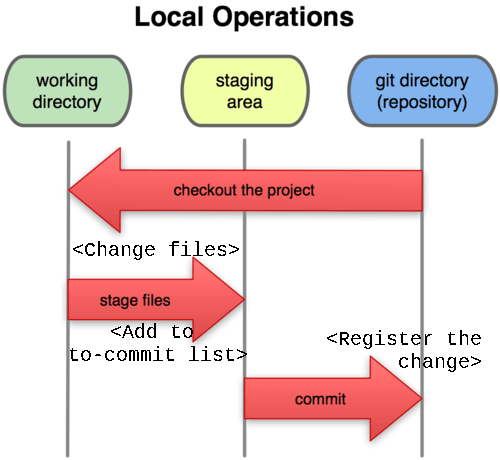
\includegraphics[width=\linewidth]{threeStates.png}
\end{frame}

\begin{frame}[plain]
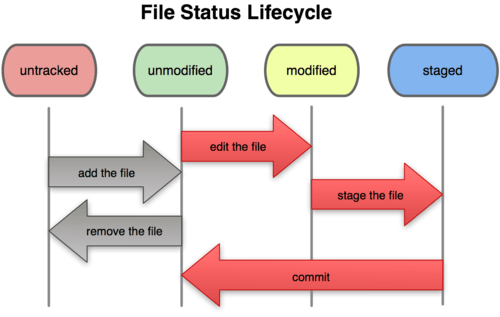
\includegraphics[width=\linewidth]{fileLifeCycle.png}
\end{frame}

\subsection{Initial commit}
\begin{frame}{Initial commit}
Applies only to an empty repository (created by git init)
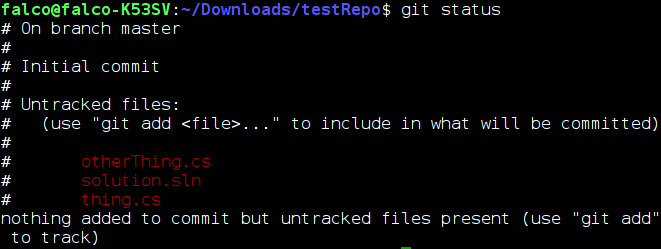
\includegraphics[width=\linewidth]{gitStatus1.png}
\end{frame}

\subsection{Adding/removing files}
\begin{frame}
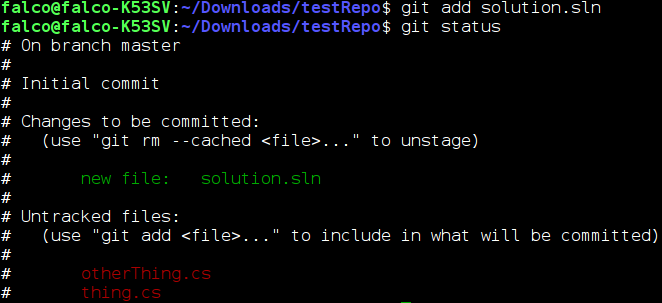
\includegraphics[width=\linewidth]{gitAdd.png}
\end{frame}

\begin{frame}
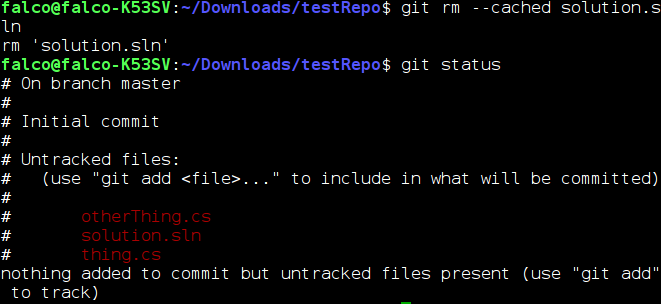
\includegraphics[width=\linewidth]{gitrmcached.png}
\end{frame}

\begin{frame}
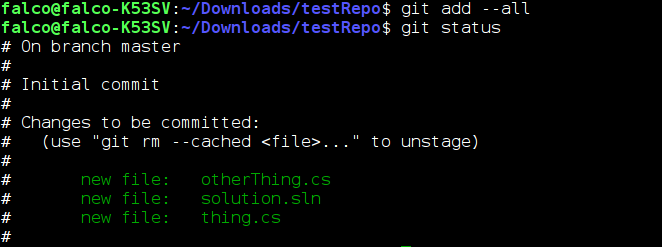
\includegraphics[width=\linewidth]{gitaddall.png}
\end{frame}

\begin{frame}
There's also:
\begin{itemize}
\item git mv file location -- Move or rename a file. Same syntax as mv command.
\item .gitignore -- a file that contains regex patterns of files that git should leave alone. Use this for executables, .obj files etc.
\end{itemize}
Tip for .gitignore files:
\url{https://github.com/github/gitignore}
\end{frame}

\subsection{Committing changes}
\begin{frame}[fragile]{Committing changes}
\begin{itemize}
\item Commit everything that's staged using git commit
\item Every commit message \textit{must} have a commit message! Tell git what you've done!
\end{itemize}
\begin{verbatim}
-- Opens vi or nano by default for the commit message:
git commit
-- Inline commit message:
git commit -m "Message here"
-- Skip staging of modified files
git commit -a -m "Message here"
git commit -am "Message here"
\end{verbatim}
\begin{itemize}
\item You cannot skip the staging of new files. Add them manually.
\end{itemize}
\end{frame}

\begin{frame}
Running the command:
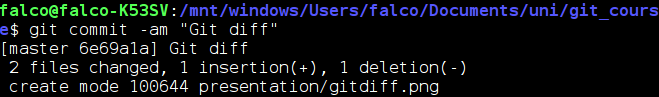
\includegraphics[width=\linewidth]{gitcommitdone.png}

Some of the info stored in the commit:
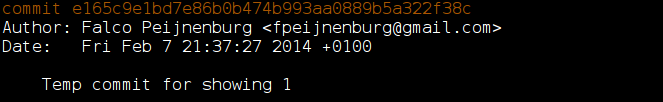
\includegraphics[width=\linewidth]{gitlogcommit.png}
\end{frame}

\section{Further commits}

\subsection{git diff}
\begin{frame}
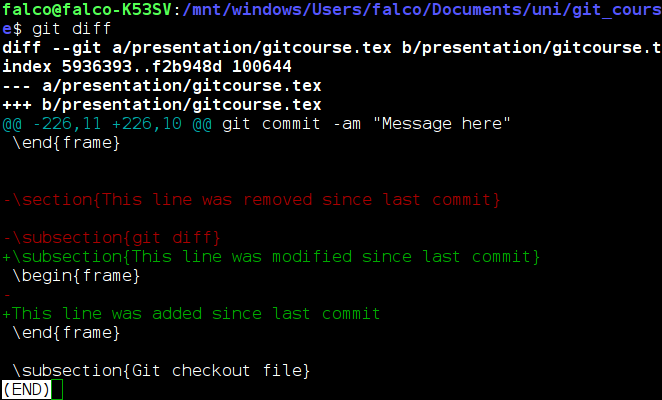
\includegraphics[width=\linewidth]{gitdiff.png}
\end{frame}

\subsection{git checkout file}
\begin{frame}{git checkout file}
\begin{itemize}
\item Undoes all the changes made to a file since last commit.
\item Doesn't leave a message
\end{itemize}
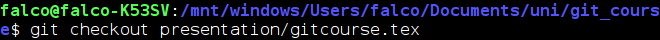
\includegraphics[width=\linewidth]{gitcheckoutfile.png}
\end{frame}

\subsection{git reset}
\begin{frame}[fragile]{git reset}
\begin{itemize}
\item useful when you've messed up the files in your working directory
\item Reset every file in your working directory to the last revision:

\begin{verbatim}
git reset --hard HEAD
\end{verbatim}
\item git reset can do many other things, but you shouldn't want to use most of those things.
\item HEAD will be explained later
\end{itemize}
\end{frame}

\subsection{git log}
\begin{frame}
git log \centerline{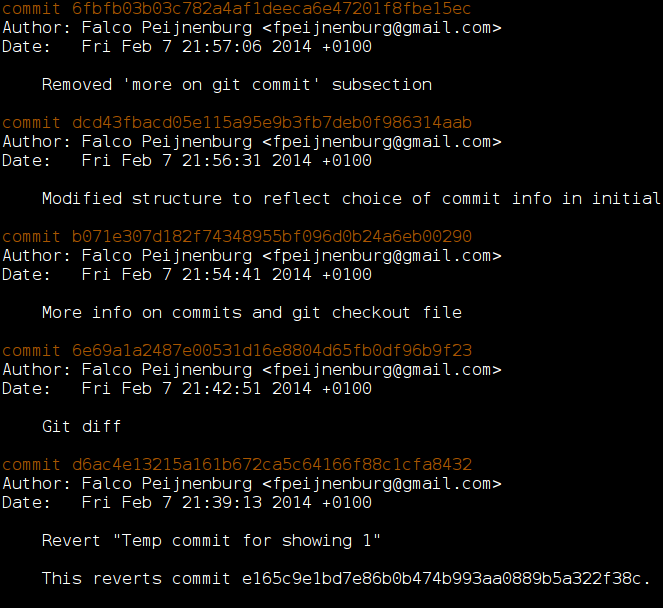
\includegraphics[width=\textheight]{gitlog.png}}
\end{frame}

\subsection{gitk}
\begin{frame}
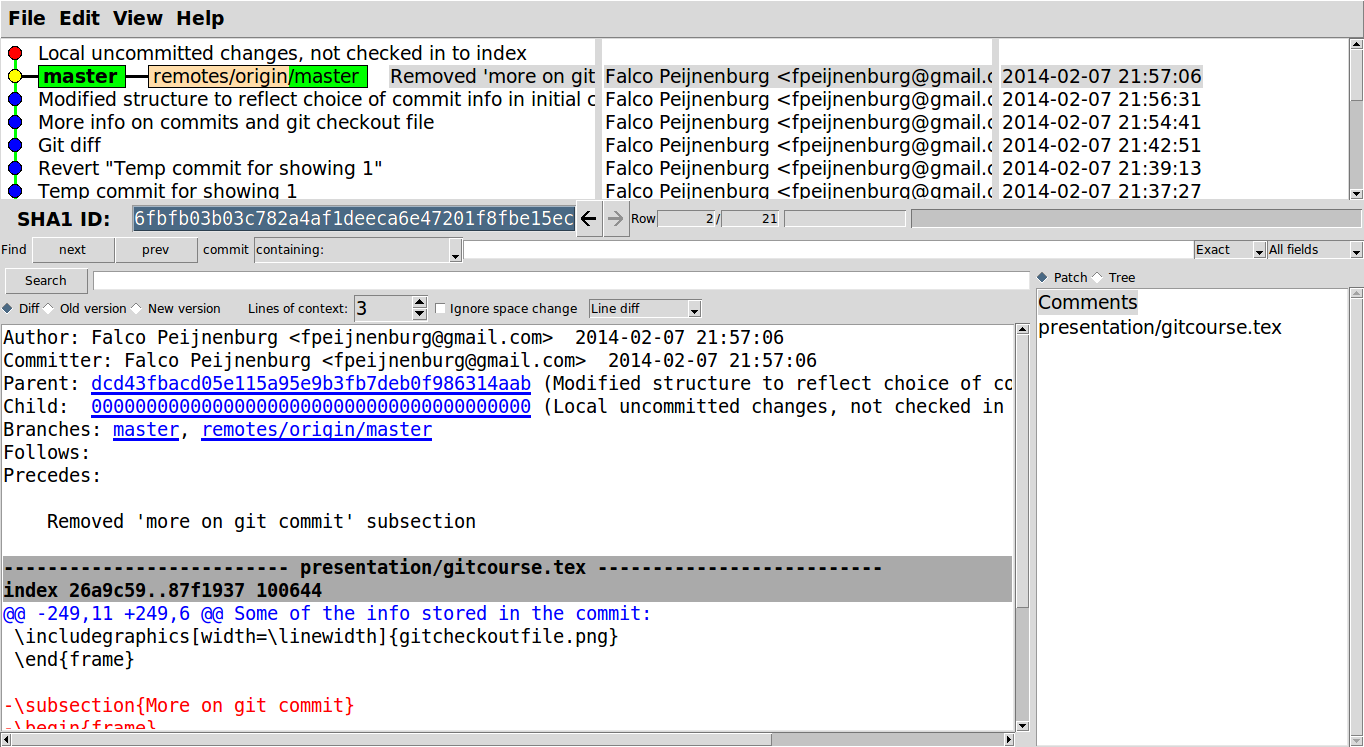
\includegraphics[width=\linewidth]{gitk.png}
\end{frame}

\subsection{git show}
\begin{frame}[fragile]{git show}
\begin{verbatim}
git show
\end{verbatim}
\begin{itemize}
\item Shows last commit information + diff
\end{itemize}

\begin{verbatim}
git show Hash_here
git show 7251b9
\end{verbatim}
\begin{itemize}
\item Shows commit info and diff of given commit
\item You can show any git object (commits, branches, stashes)
\item You don't have to use the full hash
\end{itemize}
\end{frame}


\section{The tree of commits}

\subsection{Master branch}
\begin{frame}{Master Branch}
\begin{itemize}
\item This is what we've been committing to so far.
\item Much like a linked list
\item Every commit knows its parent(s)
\end{itemize}
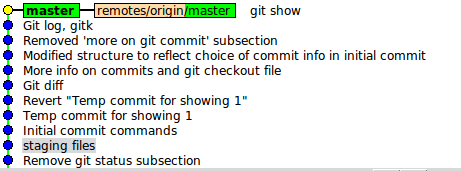
\includegraphics[width=\linewidth]{masterbranch.png}
\end{frame}

\subsection{Creating your own branch}
\begin{frame}[fragile]{Creating your own branch}
\begin{verbatim}
git branch branchname
git checkout branchname
\end{verbatim}
\begin{itemize}
\item Mind the git checkout command. It might be confusing at first.
\item Shorter:
\end{itemize}

\begin{verbatim}
git checkout -b branchname
\end{verbatim}
\begin{itemize}
\item Official definition of checkout:
\item \textit{Checkout a branch or paths to the working tree}
\end{itemize}
\end{frame}

\subsection{Switching branches}
\begin{frame}[fragile]{Switching branches}
\begin{verbatim}
git checkout master
git checkout branchname
git checkout otherBranch
\end{verbatim}
\begin{itemize}
\item You can switch from any branch to any other branch
\item Might fail if you have uncommitted changes
\end{itemize}
\end{frame}

\subsection{Merging branches}
\begin{frame}[fragile]{Merging branches}
\begin{verbatim}
git checkout mergeTo
git merge mergeFrom
\end{verbatim}
\begin{itemize}
\item Make sure you're on the right branch first
\item Conflicts may occur when merging
\item A new special merge commit will be created with \textit{two} parent commits
\item All commits from the mergeFrom branch will be visible in the mergeTo branch
\end{itemize}
\end{frame}

\subsection{Removing branches}
\begin{frame}[fragile]{Removing branches}
\begin{verbatim}
git branch -d branchname
git branch -D branchname
\end{verbatim}
\begin{itemize}
\item The former will fail if there are unmerged changes
\item The latter will not, so be careful
\end{itemize}
\end{frame}


\section{Resolving conflicts}

\subsection{What is a conflict}
\begin{frame}
\begin{itemize}
	\item Harry and Larry are working on a website
	\item Harry and Larry both edit the footer div of the main web page
	\item Harry is working on master
	\item Larry is working on the refactor branch he created
	\item After a while Larry is done working and wants to merge refactor into master
\end{itemize}
\end{frame}

\begin{frame}[fragile]
\begin{verbatim}
$ git merge refactor
Auto-merging index.html
CONFLICT (content): Merge conflict in index.html
Automatic merge failed; fix conflicts and then commit
the result.
\end{verbatim}
\begin{itemize}
	\item Two people edited the same file in the same place
	\item What should git do with that?
	\begin{itemize}
	\item Use Harry's version?
	\item Use Larry's version?
	\item Use a combination of both versions?
	\item Use neither version?
	\end{itemize}

	\item Another kind of conflict: Larry modifies a file that Harry removed. Use modified or removed?
\end{itemize}
\end{frame}

\subsection{Fixing the conflicts in the file}
% It's not a mess
\begin{frame}[fragile]{Fixing the conflicts in the file}
\begin{itemize}
\item Git will edit the files that have the conflicts
\item ``conflict markers'' will be added.
\item git status and git diff will tell you which files are conflicted.
\item Fix the conflicts in visual studio or your favourite text editor.
\item You can also set up a visual merge tool like opendiff, kdiff3, tkdiff, xxdiff, meld, \textbf{tortoisemerge}, gvimdiff, diffuse, ecmerge, p4merge, araxis, bc3, codecompare, emerge or vimdiff
\end{itemize}
\end{frame}

\begin{frame}[fragile]
\begin{verbatim}
<<<<<<< HEAD
<div id="footer">contact : email.support@github.com</div>
=======
<div id="footer">
  please contact us at support@github.com
</div>
>>>>>>> refactor
\end{verbatim}

Possible resolution:
\begin{verbatim}
<div id="footer">
  please contact us at email.support@github.com
</div>
\end{verbatim}
\end{frame}

\subsection{Registering merged file}
\begin{frame}[fragile]
\begin{verbatim}
git add fixedFile
\end{verbatim}
\begin{itemize}
\item You must add every file manually
\item Only add a file when all conflicts in it are resolved (check with git diff)

\end{itemize}
\end{frame}

\subsection{Committing the merge}
\begin{frame}

\end{frame}


\section{Remote repositories}

\subsection{Local versus remote repository}
\begin{frame}

\end{frame}

\subsection{Adding a remote repository}
\begin{frame}

\end{frame}

\subsection{Showing remote repositories}
\begin{frame}

\end{frame}

\subsection{Removing a remote repository}
\begin{frame}

\end{frame}

\subsection{Pushing and pulling}
\begin{frame}

\end{frame}


\section{Best Practices and tips}
\begin{frame}

\end{frame}


\section{Awesome things you can do with git}

\subsection{Git revert}
\begin{frame}

\end{frame}

\subsection{Submodule/Subtree merge}
\begin{frame}

\end{frame}

\subsection{Git bisect}
\begin{frame}

\end{frame}

\subsection{Git tag}
\begin{frame}

\end{frame}

\subsection{Git stash}
\begin{frame}

\end{frame}

\subsection{Git clean}
\begin{frame}

\end{frame}

\subsection{Git blame}
\begin{frame}

\end{frame}

\subsection{Pull requests}
\begin{frame}

\end{frame}

\subsection{Cherry-pick}
\begin{frame}

\end{frame}

\subsection{Set up your own git server}
\begin{frame}

\end{frame}

\section{Further reading}
\begin{frame}

\end{frame}

\end{document}